\section{The Identity-Transformation Approach}
\label{sec:challenge}

We discuss the security requirements of privacy-preserving SSO,
 and present the identity-transformation approach.


\subsection{Security Requirements of SSO}
\label{subsec:basicrequirements}

Non-anonymous SSO services~\cite{OpenIDConnect,rfc6749,SAML,SAMLIdentifier,NIST2017draft} aims to ensure a \emph{legitimate} user to login to an \emph{honest} RP using his permanent account at that RP, %correlating multiple login instances,
by presenting \emph{identity tokens} issued by a \emph{trusted} IdP. 
To achieve this goal, a trusted IdP issues an identity token~\cite{OpenIDConnect, rfc6749, SAML, SAMLIdentifier, NIST2017draft} that specifies (\emph{a}) the RP that the user requests to log in to (i.e., \emph{RP designation}) and  (\emph{b}) the user who has been authenticated by the IdP (i.e., \emph{user identification}). Thus, an honest RP verifies the designated RP identity (or pseudo-identity) in the identity tokens against its own before accepting them and authorizes the token holder to log in as the user whose (pseudo-)identity is specified in an accepted token. This prevents a malicious RP from replaying a received identity token to an honest RP and logging in as the victim user. 
The SSO login flow also requires \emph{confidentiality} and \emph{integrity} of identity tokens. An identity token must be forwarded only to the target RP by the authenticated user, and not disclosed to any other parties. Otherwise, an eavesdropper who possesses the token could successfully login to the designated RP. Maintaining integrity is also critical to prevent adversaries from tampering with a token. So, identity tokens are usually signed by a trusted IdP and transmitted over HTTPS \cite{OpenIDConnect,rfc6749,SAML}.


The sufficient and necessary conditions for secure SSO services, i.e., {\bf {\em RP designation, user identification,}} and {\bf {\em integrity and confidentiality of identity tokens}}, have been thoroughly analyzed \cite{ArmandoCCCT08, FettKS16, FettKS17}.
Any vulnerabilities that compromise any of these properties may lead to attacks~\cite{SomorovskyMSKJ12, WangCW12, ArmandoCCCPS13, ZhouE14, WangZLLYLG15, WangZLG16, YangLLZH16, MainkaMS16, MainkaMSW17, YangLCZ18, YangLS17, ShiWL19, ChenPCTKT14, ccsSunB12, DiscoveringJCS, dimvaLiM16, CaoSBKVC14, TowardsShehabM14}.


%\subsection{The Identity Dilemma of Privacy-Preserving SSO}
%\label{subsec:challenges}
\begin{table}
\footnotesize
    \caption{The (pseudo-)identities in privacy-preserving SSO}
    \centering
%    \begin{tabular}{|l|l|l|}
    \begin{tabular}{|p{1.0cm}|p{5.1cm}|p{1.13cm}|} \hline
    {\textbf{Notation}} & {\textbf{Description}} & {\textbf{Lifecycle}} \\ \hline
    {$ID_U$} & {The user's unique identity at the IdP.} & {Permanent} \\ \hline
    {$ID_{RP_j}$} & {The $j$-th RP's unique identity at the IdP.} & {Permanent} \\ \hline
    {$PID_{U,j}^i$} & {The user's pseudo-identity, in the user's $i$-th login instance to the $j$-th RP.} & {Ephemeral} \\ \hline
    {$PID_{RP_j}^i$} & {The $j$-th RP's pseudo-identity, in the user's $i$-th login instance to this RP.} & {Ephemeral} \\ \hline
    {$Acct_j$} & {The user's identity (or account) at the $j$-th RP.} & {Permanent} \\ \hline
    \end{tabular}
    \label{tbl:notations-dilemma}
\end{table}

\subsection{Identity Transformation}
\label{subsec:solutions}

\textcolor{blue}{We aim to design a privacy-preserving SSO system with the four security properties as above,
    while preventing both the IdP-based login tracing and the RP-based identity linkage.
%We explicitly distinguish a user's identity (or \emph{account}) at an RP,
%     from the user's \emph{identity} at an IdP and the user's \emph{pseudo-identities} enclosed in identity tokens.
In UPPRESSO these requirements are satisfied through \emph{transformed identities} in the identity tokens.
Table \ref{tbl:notations-dilemma} lists the notations in the following explanations,
    and the subscript $j$ and/or the superscript $i$ may be omitted when there is no ambiguity.}

\textcolor{blue}{In an SSO login flow, % with identity transformations,
    a user firstly negotiates \emph{ephemeral} $PID_{RP}$ with a target RP,
and sends an identity-token request enclosing $PID_{RP}$ to an IdP.
After authenticating the user as $ID_U$, the IdP calculates \emph{ephemeral} $PID_U$ based on $ID_U$ and $PID_{RP}$,
    and issues an identity token binding $PID_U$ and $PID_{RP}$.
On receiving a token with matching $PID_{RP}$,
    the RP calculates \emph{permanent} $Acct$ and allows the token holder to login as $Acct$.
%
%Given a user,
%    (\emph{a}) an identity token contains only pseudo-identities, i.e., $PID_{U,j}^i$ and $PID_{RP_j}^i$,
%        which are independent of each other for different RPs and in multiple login instances, respectively,
%    and (\emph{b}) these \emph{ephemeral} pseudo-identities enable the target RP to derive a \emph{permanent} account, i.e., $Acct_j$.
The relationship among (pseudo-)identities is illustrated in Figure \ref{fig:IDCorrelation}.
The \emph{red} and \emph{green} blocks represent \emph{permanent} and \emph{ephemeral} (pseudo-)identities, respectively.
The labeled arrows denote the transformations of (pseudo-)identities.}
%It describes the {\em identity dilemma} of privacy-preserving SSO as below:

%An identity token binds the (pseudo-)identities of an authenticated user and an RP.
%Since an IdP authenticates users and then always knows the user's identity (i.e., $ID_U$),
%    to prevent the IdP-based login tracing,
%    we should not reveal the target RP's permanent identity (i.e., $ID_{RP}$) to the IdP.

\textcolor{blue}{To ensure RP designation,
     $PID_{RP}$ should be \emph{uniquely} associated with the target RP.
To ensure user identification,
    an \emph{ephemeral} $PID_{U}^i$ in each login instance should enable the RP to derive a \emph{permanent} account  (i.e., $Acct$) at this RP.}


%An \emph{ephemeral} pseudo-identity for the RP (i.e., $PID_{RP}$) is used in the identity-token request:
\textcolor{blue}{To prevent the IdP-based login tracing,
    the IdP does not obtain any information about $ID_{RP}$ from any $PID_{RP}^i$,
        thus, in multiple login instances to a given RP,
           (\emph{a})  $PID_{RP}^i$ should
         be independent of each other,\footnote{Even when the target RP is kept unknown to the IdP,
            the IdP should not link multiple login instances to this RP.}
   % the IdP-based login tracing is still effective, to correlate a user's multiple login instances.
and  (\emph{b}) %to a given RP,
 $PID_U^i$ should be independent of each other.\footnote{If $PID_U^i$ is not completely independent of each other,
         it implies the IdP could link multiple login instances to a given RP.}
To prevent the RP-based identity linkage,
% the IdP does not enclose $ID_U$ in identity tokens.
%a user pseudo-identity (i.e., $PID_U$) is bound instead:
%$PID_U$ is bound in identity tokens:
    the RP does not obtain any information about $ID_U$ from any $PID_{U,j}$,
    which implies $PID_{U,j}$ for different RPs should be independent of each other.}

\begin{figure}[bt]
  \centering
  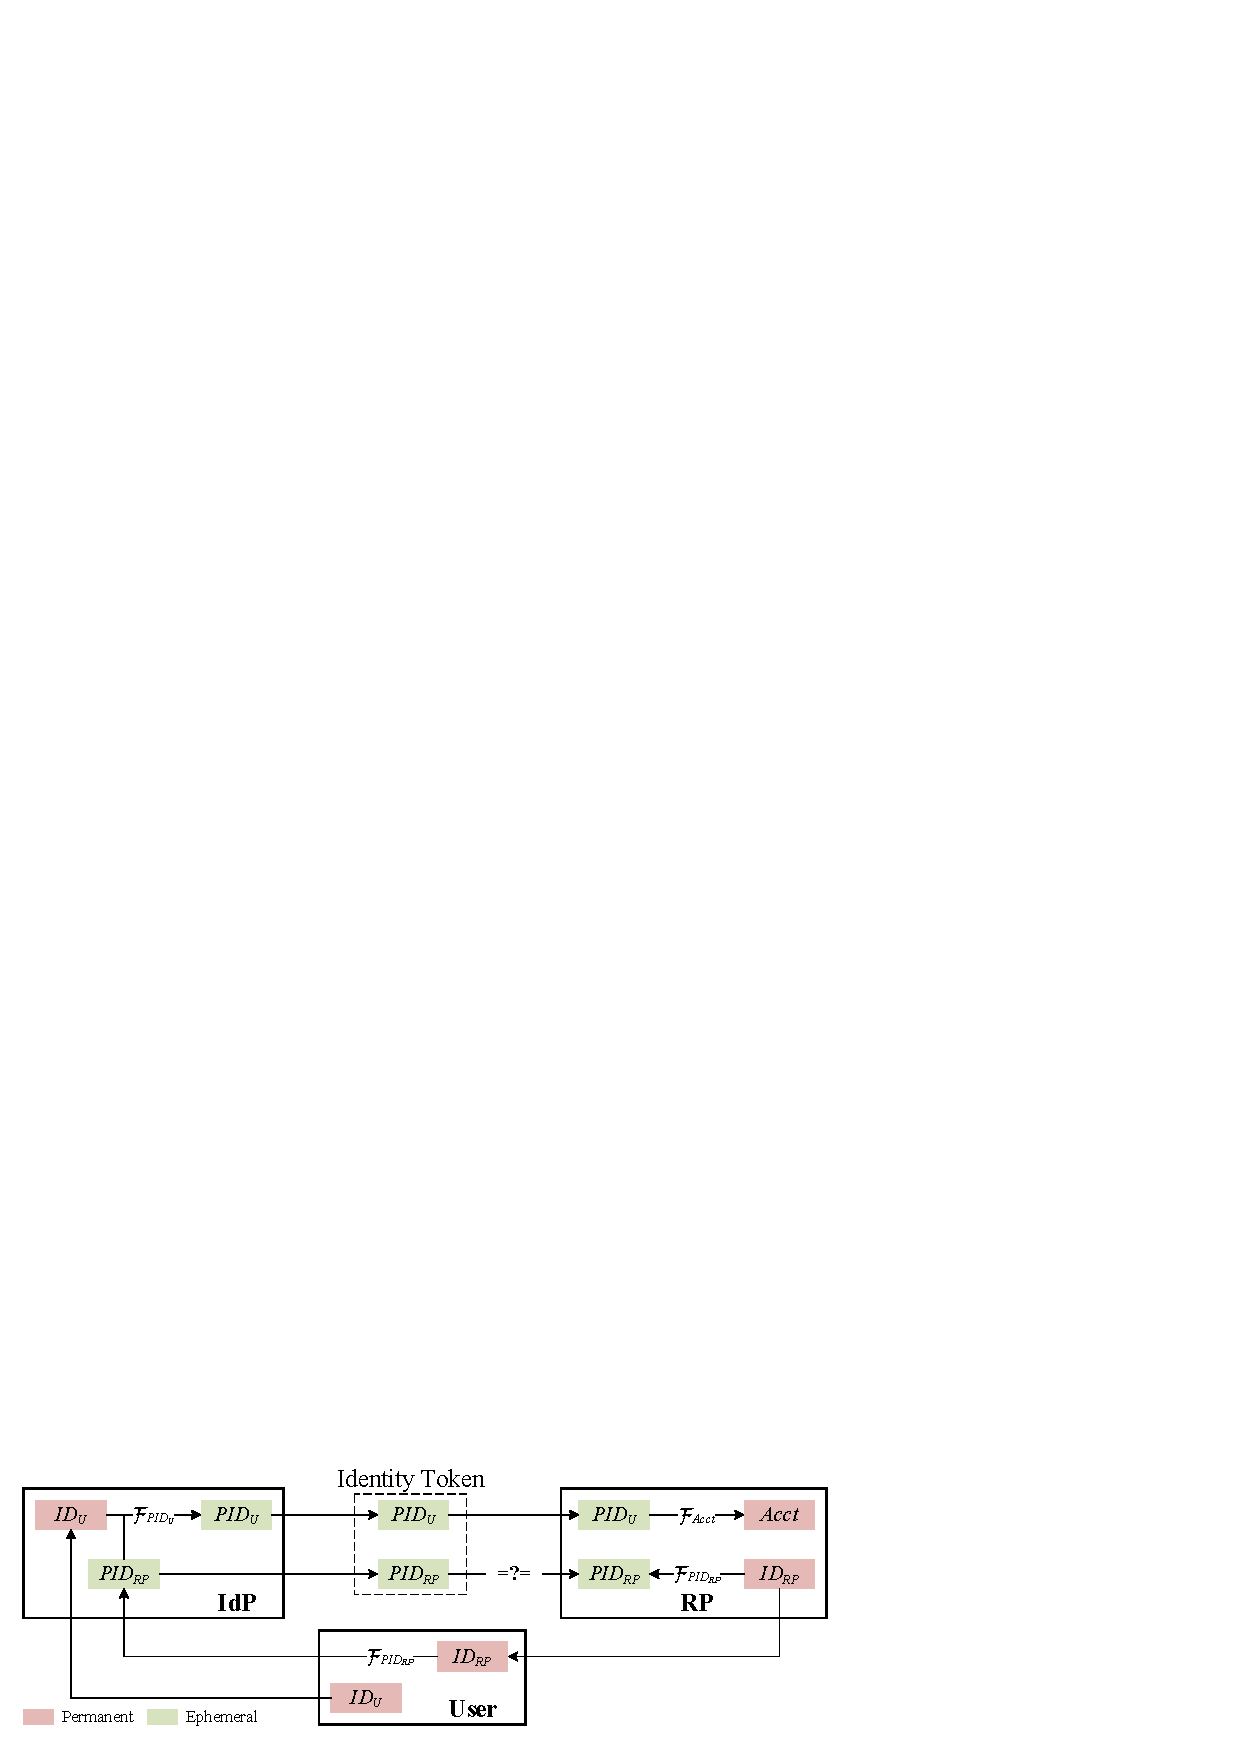
\includegraphics[width=0.99\linewidth]{fig/IDCorrelation.pdf}
  \caption{Identity transformations in privacy-preserving SSO}
  \label{fig:IDCorrelation}
\end{figure}

%We pose the \emph{identity dilemma} (or challenge) of SSO identity tokens
%    to satisfy the requirements of both security and privacy:
%
%\noindent\emph{Given an authenticated user and an unknown RP (i.e., permanent $ID_U$ and ephemeral $PID_{RP}$),
%    an IdP is expected to generate an ephemeral pseudo-identity (i.e., $PID_{U}$)
%     which will be correlated with the user's permanent identity at this RP (i.e., $Acct$),
%     while knowing nothing about the RP's identity or the user's account at this RP (i.e., $ID_{RP}$ or $Acct$).}

%Existing privacy-preserving SSO solutions (i.e., SPRESSO \cite{SPRESSO}, BrowserID \cite{BrowserID} and PPID \cite{NIST2017draft})
%  do not explicitly and comprehensively consider all five (pseudo-)identities in the SSO login flow,
%    and $ID_U$ or $ID_{RP}$ is still enclosed in identity tokens.
%So only one type of privacy threat is prevented.

\textcolor{blue}{The following identity transformations %in a login flow
    are needed: %in UPPRESSO.
\vspace{-\topsep}\begin{itemize}
\setlength{\topsep}{0pt}
\setlength{\partopsep}{0pt}
\setlength{\itemsep}{0pt}
\setlength{\parsep}{0pt}
\setlength{\parskip}{0pt}
\item
$\mathcal{F}_{PID_{RP}}(ID_{RP}) = PID_{RP}$, calculated by the user and the RP.
From the IdP's view,
$\mathcal{F}_{PID_{RP}}()$ is a one-way function and $PID_{RP}$
is \emph{indistinguishable} from random variables.
\item
$\mathcal{F}_{PID_U}(ID_U, PID_{RP}) = PID_{U}$, calculated by the IdP.
From the target RP's view,
    $\mathcal{F}_{PID_U}()$ is a one-way function and $PID_{U}$ is \emph{indistinguishable} from random variables.
\item
$\mathcal{F}_{Acct}(PID_{U}, PID_{RP}) = Acct$, calculated by the RP.
Given $ID_U$ and $ID_{RP}$, $Acct$ is \emph{permanent} and \emph{unique} to other accounts at this RP.
In a user's any $i$-th and $i'$-th ($i \neq i'$) login instances to the RP,
 $\mathcal{F}_{Acct}(PID_{U}^i, PID_{RP}^i) = \mathcal{F}_{Acct}(PID_{U}^{i'}, PID_{RP}^{i'})$.
\end{itemize}}

